\subsection{(1) Influence of Different \texorpdfstring{$\mu$}{mu} Values on the Regret}

For each of the three values $\mu \in \{0.25,0.375,0.4375\}$, we generated i.i.d.\ Bernoulli($\mu$) sequences of length $T=2000$ (with 10 runs). In Figure~\ref{fig:plots_iid}, we show the pseudo-regret over time for FTL and the different Hedge variants. The final average pseudo-regrets at $t=2000$ are:
\begin{verbatim} 
Final average pseudo-regret at t=2000 for p=0.25: 
FTL: 0.200 
Hedge_fixed(0.026327688477341595): 26.000 
Hedge_fixed(0.05265537695468319): 13.400 
Hedge_anytime(1.0): 4.600 
Hedge_anytime(2.0): 1.400

Final average pseudo-regret at t=2000 for p=0.375: 
FTL: 1.800 
Hedge_fixed(0.026327688477341595): 26.800 
Hedge_fixed(0.05265537695468319): 15.500 
Hedge_anytime(1.0): 13.800 
Hedge_anytime(2.0): 5.700

Final average pseudo-regret at t=2000 for p=0.4375: 
FTL: 5.100 
Hedge_fixed(0.026327688477341595): 29.700 
Hedge_fixed(0.05265537695468319): 13.100 
Hedge_anytime(1.0): 20.300 
Hedge_anytime(2.0): 11.700 
\end{verbatim}

From these results, we see that smaller $\mu$ generally yields lower final pseudo-regret for FTL, while Hedge’s performance depends heavily on its learning rate ($\eta$). Larger learning rates can hurt Hedge if $\mu$ differs significantly from $0.5$, but the “anytime” versions tend to adapt better over time.

\begin{figure}[h!] 
    \centering 
    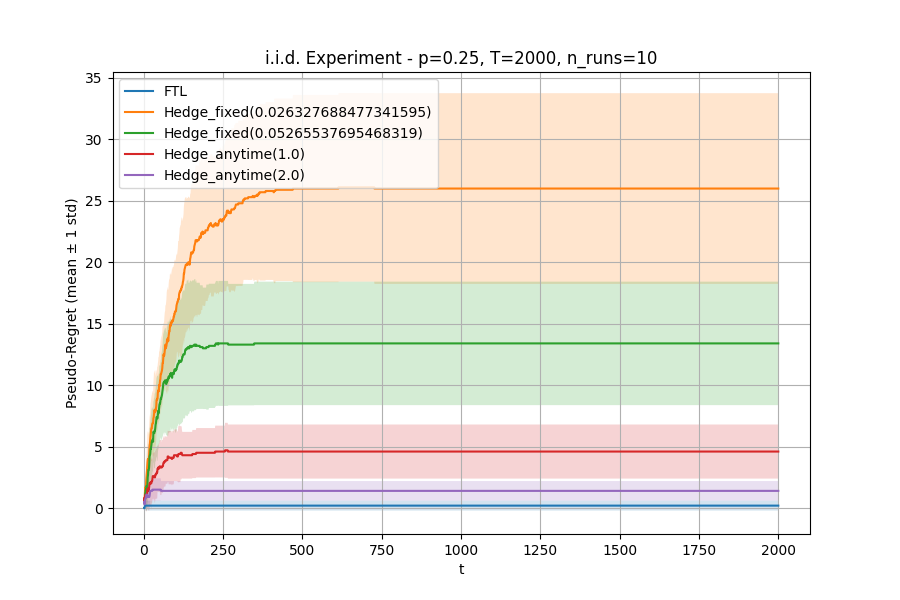
\includegraphics[width=0.65\textwidth]{Code/Figure_1.png}
    \caption{Example pseudo-regret curves for i.i.d.\ data with $\mu=0.25$.} 
    \label{fig:plots_iid} 
\end{figure}

\subsection{(2) Adversarial Sequence Design and Results}

We designed an adversarial sequence by letting:
\begin{lstlisting}[language=Python, caption={Adversarial sequence alternating 0 and 1.}] 
def simulate_adversarial_sequence(T): 
    return np.array([t % 2 for t in range(1, T+1)]) 
\end{lstlisting} 

This sequence forces frequent switches if the algorithm tries to follow whichever label occurred more often so far. We ran the same 10 repetitions (the randomness comes from Hedge’s sampling) and computed the \emph{regret} (algorithm’s loss minus the best constant expert’s loss) at each time $t$. The final average regret at $t=2000$ is:

\begin{verbatim} 
Final average regret at t=2000 (adversarial): 
FTL: 1000.000 
Hedge_fixed(0.026327688477341595): -3.200 
Hedge_fixed(0.05265537695468319): 29.900 
Hedge_anytime(1.0): 16.200 
Hedge_anytime(2.0): 13.500 
\end{verbatim}

We observe that FTL’s regret is very large (around 1000), while some versions of Hedge achieve much smaller or even negative regret. This confirms that in certain adversarial designs, FTL can perform significantly worse than Hedge.

\begin{figure}[h!] 
    \centering 
    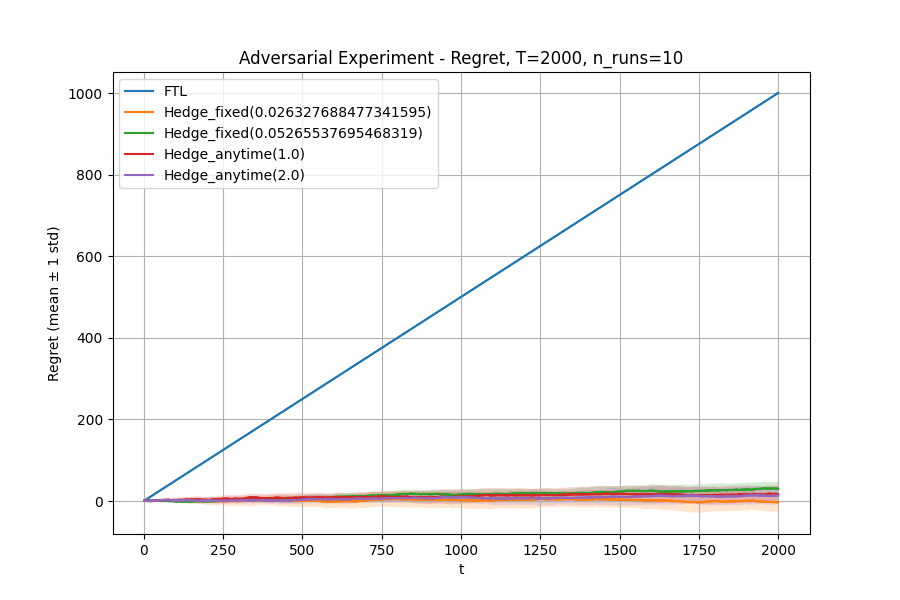
\includegraphics[width=0.65\textwidth]{Code/Figure_4_adversarial.png}
    \caption{Regret over time on the adversarial sequence.} 
    \label{fig:plots_adversarial} 
\end{figure}

\subsection{(3) Code Snippets and Observations}

Below are the key code snippets for \texttt{FTL} and \texttt{Hedge} used in the experiments:

\begin{lstlisting}[language=Python, caption={FTL implementation.}] 
def ftl_predict(X): 
    T = len(X) 
    cum_loss = np.zeros(T) 
    L0, L1 = 0, 0 
    mistakes = 0 
    for t in range(T): 
        if L0 < L1: 
            pred = 0 
        elif L1 < L0: 
            pred = 1 
        else: 
            pred = 0 
        if pred != X[t]: 
            mistakes += 1 
        if X[t] == 1: 
            L0 += 1 
        else: 
            L1 += 1 
        cum_loss[t] = mistakes 
    return cum_loss 
\end{lstlisting}

\begin{lstlisting}[language=Python, caption={Hedge implementation.}] 
def hedge_predict(X, schedule_type, param): 
    T = len(X) 
    L = np.zeros(2) 
    cum_loss = np.zeros(T) 
    mistakes = 0 
    for t in range(1, T+1): 
        if schedule_type == 'fixed': 
            eta_t = param 
        else: 
            eta_t = param * np.sqrt(np.log(2)/t) 
        L_min = np.min(L) 
        w = np.exp(-eta_t * (L - L_min)) 
        p = w / np.sum(w) 
        action = np.random.choice([0, 1], p=p) 
        if action != X[t-1]: 
            mistakes += 1 
        loss0 = 1 if X[t-1] == 1 else 0 
        loss1 = 1 if X[t-1] == 0 else 0 
        L[0] += loss0 
        L[1] += loss1 
        cum_loss[t-1] = mistakes 
    return cum_loss 
\end{lstlisting}

From these plots and results, we can see how the Hedge algorithm adapts better to adversarial changes, whereas FTL fails in the adversarial sequence. For the i.i.d.\ case, FTL often remains competitive, especially when $\mu$ is small, but Hedge can outperform it with properly tuned parameters.
